\documentclass[
    titlepage,
    twoside,
    openright,
    12pt
]{book}

\usepackage{lib/polithesis}

%*****************************************************************
%                         CUSTOM PACKAGES                         
%*****************************************************************

% Should you need to add custom packages, this is the right place.

%*****************************************************************
%                      THESIS CUSTOMIZATIONS                      
%*****************************************************************
%
%   In this section, you can insert the data to be displayed in
%   the title page. If you do not want to show something, just
%   comment it using '%' at the beginning of the line.
%
%*****************************************************************

% Specify thesis language in lowercase (default "english")
\thesislanguage{english}
% Choose the font for the thesis
% The available choices are: "Computer Modern", "Baskerville",
% "Nimbus", "Palatino", "Utopia".
% If an invalid font is set, the fallback font used is the default
% LaTeX font "Computer Modern".
\thesisfont{Palatino}
% Change title color
\titlecolor{MidnightBlue}
% Change color of chapters' number
\chapnumbercolor{ThesisGray}
% The available colors are the 68 dvips colors plus the defaults.
% (https://en.wikibooks.org/wiki/LaTeX/Colors#Predefined_colors)
% You can define you own color as done for ThesisGray in the
% library file, even if it is not recommended.

%*****************************************************************
%                         TITLE PAGE DATA                         
%*****************************************************************
%
%   In this section, you can insert the data to be displayed in
%   the title page. If you do not want to show something, just
%   comment it using '%' at the beginning of the line.
%
%*****************************************************************

\university{Politecnico di Milano}
\faculty{Facoltà di Ingegneria}
\school{Scuola di Ingegneria Industriale e dell'Informazione}
\department{Dipartimento di Elettronica, Informazione e
 Bioingegneria}
\course{Computer Science and Engineering}
\title{A Fancy Title\\for a Fancy Thesis}
\supervisor{Prof. Enrico Fermi}
% You can specify more than one co-supervisor, separating them
% with commas.
\cosupervisors{Prof. Alice First, Dr. Bob Second}
% Each author should be added as a tuple of her name and her
% matriculation number joined with a comma.
% You can specify more than one author, separating each one with
% a comma. They will be printed in different lines.
\authors{Your Self, 000000, Your Second Self, 111111}
\matriculationPrefix{matr.}
\academicYear{20MM/20MN}

%*****************************************************************
%                         THESIS CONTENT                         
%*****************************************************************

\begin{document}

% Title Page
\maketitle

% Optional, comment or delete instruction to remove
\dedication{Insert here your dedication.\\Optional.}

% Chapters
\frontmatter
\pagenumbering{Roman}
\chapter{Abstract}

Here goes the abstract, a summary of your thesis work. You may add some keyword at the end that clearly identify the research field of the thesis. The abstract should not contain any reference to related works.

\paragraph{Keywords}  keyword1; keyword2; keyword3
\chapter{Sommario}
In questo capitolo puoi inserire l'abstract della tesi in italiano.

\paragraph{Parole chiave} keyword1; keyword2; keyword3
\chapter{Acknowledgements}
In this chapter, you can acknowledge the people that were somehow helpful in the realization of the thesis. It is better to keep this chapter formal, you can add the friendly thanks at the end (chapter Thanks).
\thesistoc

%*****************************************************************
%                            CHAPTERS                            
%*****************************************************************

\mainmatter
\chapter{Introduction}

\section{Context}
This is basically an extension of the abstract. Here you provide context for the problem faced. Keep in mind that even if you now have gained expertise on it, most of the readers are no so inside the problem as you are. Start from the basics and explain clearly. You can also introduce here some hints about the methodology and your contribution. For this purpose, you may also decide to add more sections.

\section{Thesis outline}
Here you explain the structure of the thesis.

\begin{example}
The thesis is structured in the following way:
\begin{itemize}
\item In \autoref{ch:preliminaries_and_sota}, we present ... .
\item In \autoref{ch:problem_formulation}, we formulate the problem we address in the thesis and ... .
\item In \autoref{ch:design}, we present our solution for ... .
\item In \autoref{ch:experiments}, we show experimental results of our proposed methods in different settings ... .
\item Finally, in \autoref{ch:conclusions}, we present our conclusions and possible future paths toward which our work could be extended.
\end{itemize}
\end{example}

\chapter{Preliminaries and State of the Art}
\label{ch:preliminaries_and_sota}

\section{Preliminary notions}
\label{sec:preliminaries}

\begin{table}[!ht]
\centering
\begin{tabular}{c l} \hline
\textbf{Notation}&\textbf{Description} \\ \hline
$G$&Graph\\
$V$&set of nodes of $G$\\
$E$&set of edges of $G$\\
$W$&set of weights corresponding to each edge in $E$\\
$w_{u,v}$&weight of edge $(u,v)$\\
$n$&$|V|$, number of nodes\\
$m$&$|E|$, number of edges\\
\hline
\end{tabular}
\caption{Graph notation.}
\label{tab:notation}
\end{table}

``In this section, we introduce the preliminary notions at the base of our study. We start by briefly introducing the problem, and then we provide the necessary concepts and the notation used."

You may insert a subsection for each of the most relevant features of your problem. You can add some reference if needed, but just to explain the problem. The references with the solutions of the problem should be put in the next section.

You can keep a notation table for the notation used in this chapter as \autoref{tab:notation}. Everything inside the notation table must be written at least once inside this chapter. You can put an extended notation for the whole thesis in the appendix.

It is likely that you have to present definitions, theorems or propositions. We suggests to use the environments provided by the template. You can find the guide in the LaTeX suggestions chapter.

\section{State of the Art}
\label{sec:sota}

In this section, we survey the most relevant works related to the argument of your thesis. If you face a problem that has more than one macro-topic, you may choose to add a subsection for each of these topics (better no more than 2-3), like \emph{Related works on Topic 1}, etc.

List the works in chronological order and cite only the most important and pertinent ones, avoid 100 citations for a master thesis.
\chapter*{\LaTeX~ suggestions}

\begin{center}
\bfseries 
\color{red}{REMOVE THIS CHAPTER BEFORE SUBMISSION}
\end{center}

\noindent In this file there are listed some tips you may find useful. Some of the shortcuts shown are custom, so I suggest you to have a look at what's next even if you are expert in LaTeX.

\section*{Math}

All the fonts supported by the template provide a math variant for the formulas. You can use the standard math commands of LaTeX plus the following additions:
\begin{itemize}
\item Argmin/max: $\argmin_i$, $\argmax_i$, and their rendering in centered equations
$$\argmin_i \quad \argmax_i$$
\item Variance: $\var$, $\Var{p}$
\item Expected value: $\ev$, $\Ev{p}$
\end{itemize}

\section*{Custom commands}

We provide two commands you may find useful.

The command \texttt{\textbackslash blankpage} adds a blank page. Differently from \texttt{\textbackslash newpage}, the added page is completely blank and the text resume from the page after.

The command \texttt{\textbackslash todo} let you add the \todo symbol in the text. You can use it whenever you have text to be revisioned after.

\section*{Environments}

The thesis package provide three useful packages you may need for the theoretical part.

\subsection*{Definition}

Definitions are used for introducing a concept and its theoretical meaning for the first time. Do not use it just for clarifying the notation. Definitions are numbered within the chapter, such that the first definition of chapter 2 is 2.1. The syntax is the following:
\begin{verbatim}
\begin{definition}[NAME (optional)]
\label{def:LABEL}
DEFINITION
\end{definition}
\end{verbatim}

\noindent Example:

\begin{definition}[$(\alpha, \beta)$-approximation]
\label{def:alphabetaapprox}
An $(\alpha, \beta)$\textit{-approximation} algorithm outputs with success probability $\beta$ a solution which is at least $\alpha$ fraction of the optimal solution, for some $\alpha, \beta \leq 1$.
\end{definition}

\subsection*{Theorem}

Theorems are numbered incrementally within the thesis, regardless of the chapter they are declared in. The syntax is the following:
\begin{verbatim}
\begin{theorem}
\label{thm:LABEL}
THEOREM
\end{theorem}
\end{verbatim}

\noindent Example:

\begin{theorem}
\label{thm:approximation}
For a non-negative, monotone, submodular function $f(\cdot)$, let $S_k$ be a set obtained by selecting $k$ elements one at a time, each time choosing an element that provides the largest marginal increase in the function value. Let $S_k^*$ be a set that maximizes the value of $f(\cdot)$ over all $k$-sized sets. Then,
$$f(S_k) \geq \left( 1-\frac{1}{e} \right) \cdot f(S_k^*).$$
\end{theorem}

\subsection*{Lemma}
Lemma are like theorems. The syntax is the following:
\begin{verbatim}
\begin{lemma}
\label{thm:LABEL}
LEMMA
\end{lemma}
\end{verbatim}

\noindent Example:

\begin{lemma}
\label{thm:lemma}
This is a lemma.
\end{lemma}

\subsection*{Proposition}
Propositions are like lemmas but they are numbered within the chapter. The syntax is the following:
\begin{verbatim}
\begin{proposition}
\label{thm:LABEL}
PROPOSITION
\end{proposition}
\end{verbatim}

\noindent Example:

\begin{proposition}
\label{thm:chernoff}
If the diffusion process starting with $S$ is simulated independently at least $r=\Omega\left(\frac{n^2}{\varepsilon^2}\ln\left(\frac{1}{\delta}\right)\right)$ times, then the average number of activated nodes over these simulations is a $(1 \pm \varepsilon)$-approximation to $\sigma(S)$, with probability at least $1 - \delta$.
\end{proposition}

\subsection*{Algorithm}
The algorithm environment is used to show pseudocodes. The syntax, which follows the same paradigm of table/tabular combo, is the following:
\begin{verbatim}
\begin{algorithm}[FLOATING OPTIONS]
\caption{CAPTION}
\label{alg:LABEL}
\begin{algorithmic}[1 if you want the lines to be numbered]
ALGORITHM
\end{algorithmic}
\end{algorithm}
\end{verbatim}

\noindent Example:

\begin{algorithm}[H]
\caption{Combinatorial Thompson Sampling}
\label{alg:cts}
\begin{algorithmic}[1]
\Require Directed graph $G(V,E)$, budget constraint $k$, time horizon $T$
\For {$i = 1$ \textbf{to} $|E|$}
\State $\alpha_i = 1, \beta_i = 1$ \Comment{Assign a Beta distribution Beta(1,1) to each edge}
\EndFor

\For {$t = 1$ \textbf{to} $T$}
\State For each arm $i$, draw a sample $\theta_i(t) \sim$ Beta$(\alpha_i, \beta_i)$
\State Let $\boldsymbol{\theta}(t) = \left(\theta_1(t), \ldots, \theta_m(t) \right)$
\State $S_t \gets$ \texttt{oracle}$(G(V,E,\boldsymbol{\theta}(t)), k)$
\State Run cascade with $S_t$ as the seed set and collect the feedback $F_t$
\State Update the Beta distributions of the edges involved using $F_t$
\EndFor
\end{algorithmic}
\end{algorithm}

\section*{Referencing}

All the declared environments above can be referenced using the \texttt{{\textbackslash autoref}} command. \autoref{def:alphabetaapprox}, \autoref{thm:approximation}, \autoref{thm:chernoff}, \autoref{alg:cts}.
\chapter{Problem formulation}
\label{ch:problem_formulation}

This chapter is dedicated to the formal presentation of the problem with the technical details. Here your should put also the figure of merit you use to compare your solution with the ones of the related works you presented.

``In this thesis, we address the problem of ..."

``The figure of merit ..."

\chapter{Design and Implementation}
\label{ch:design}

``This approach is similar to the one proposed in a recent work by Nuara et al.~\cite{nuara2020driving}, in which ..."
\chapter{Experimental evaluation}
\label{ch:experiments}

``In this chapter, we present experimental results on the algorithms proposed and we compare them with state of the art methods." 

\section{Experimental setting}

\begin{table}[ht]
\centering
\renewcommand{\arraystretch}{1.2}
\begin{tabular}{|l|c|c|c|c|c|}\hline
\textbf{Name}&$n$&$m$&Average degree&Max $In(v)$&Max $Out(v)$\\ \hline\hline
Email&971&3466&3.57&4&47\\ \hline
\end{tabular}
\caption{Dataset used for the experiment.}
\label{tb:elf_datasets}
\end{table}

\paragraph{Datasets} \autoref{tb:elf_datasets} shows the characteristics of the dataset used for the experiment. The dataset is a subgraph obtained from a real dataset provided by SNAP \cite{snapnets}, \emph{email-Eu-core}, generated using email data from a large European research institution. A directed edge $(u, v)$ means that person $u$ sent an e-mail to person $v$.

As widely done in literature, we assigned the ground-truth influence probabilities according to the weighted cascade model, that is, $p_{u,v}=\frac{1}{|In(v)|}$, for each edge $(u,v) \in E$.

\paragraph{Algorithms}

For the learning process, we use the Thompson Sampling (TS) as principal exploration strategy (\autoref{alg:cts}). For the sake of completeness, we show also results with a Pure Exploitation (PE) approach, in which the oracle is fed with the mean estimates of the influence probabilities at each round.

\section{Results}

\paragraph{Experiment 1}
In this experiment, we test the algorithms on Email over a time horizon of $T=100$ rounds. The objective is to show the performances of the algorithms. The results have been averaged over 30 runs. \autoref{fig:exp_email} shows the cumulative regret, with a 95\% confidence interval.

\begin{figure}[H]
  \centering
  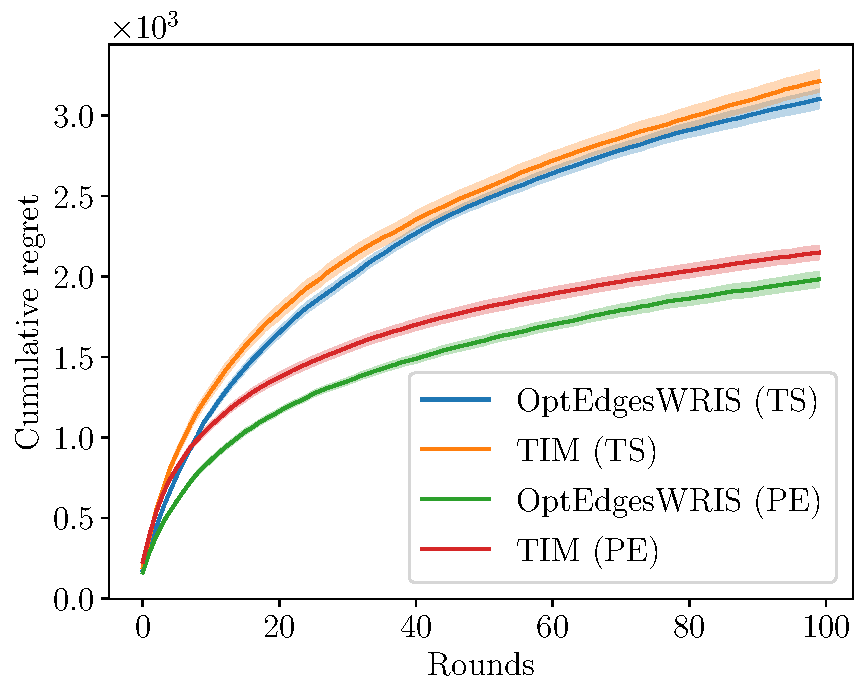
\includegraphics[width=.65\textwidth]{experiments/regret.pdf}
\caption{Cumulative regret in Email-In4 with 95\% confidence interval.}
\label{fig:exp_email}
\end{figure}

As shown in the plot, our algorithm performs better with both the exploration strategies. However, the gain on TIM is more evident with the PE strategy, specially in the first rounds.
\chapter{Conclusions and Future Works}
\label{ch:conclusions}

In this chapter, you present the conclusions of your thesis and a couple of possible future works to extend your results. First of all, you should briefly repeat the problem you addressed in the thesis. Then, you report your achievements and how they improve the state of the art.

\section{Conclusions}
``In this thesis, we analyzed ..."\\
``We proposed a new approach that ..."\\
``We tested this method on ..."\\
``Reported results show that our proposal outperforms the state of the art method."

\section{Future works}
``There are several appealing paths for future works ... ."\\
``A possible extension could be to ..."


%*****************************************************************
%                            APPENDIX                            
%*****************************************************************

\appendix
\chapter{Notation}

\begin{table}[H]
\centering
\begin{tabular}{c l} \hline
\textbf{Notation}&\textbf{Description} \\ \hline
$G$&influence graph\\
$V$&set of nodes of $G$\\
$E$&set of edges of $G$\\
$W$&set of influence weights corresponding to each edge in $E$\\
$w_{u,v}$&weight of edge $(u,v)$\\
$n$&$|V|$, number of nodes\\
$m$&$|E|$, number of edges\\
\hline
\end{tabular}
\caption{Notation used.}
\label{tab:thesis_notation}
\end{table}
\chapter*{Acknowledgments}
Here you can insert optionally the acknowledgments for who had a significant importance for the accomplishment of this goal. These acknowledgments are less formal than the ones at the beginning of the thesis and are not listed in the table of contents.

%*****************************************************************
%                         REFERENCE LIST                         
%*****************************************************************

\bibliography{biblio}

\end{document}